

\documentclass[journal]{IEEEtran}

%%%%%%%%%%%%%%%%%%%%%%%%%%%%%%%%%%%%%%%%%%%%%%%%%%%%%%%%%%%%%%

\usepackage[italian]{babel}

% *** CITATION PACKAGES ***
\usepackage[style=ieee]{biblatex} 
\bibliography{digital.bib}    %your file created using JabRef
\usepackage{hyperref}

% *** MATH PACKAGES ***
\usepackage{amsmath}
 \usepackage{multirow}

% *** PDF, URL AND HYPERLINK PACKAGES ***
\usepackage{url}
% correct bad hyphenation here
\hyphenation{op-tical net-works semi-conduc-tor}
\usepackage{graphicx}  %needed to include png, eps figures
\usepackage{float}  % used to fix location of images i.e.\begin{figure}[H]

\usepackage{csquotes} % correzione errore compilazione

%%%%%%%%%%%%%%%%%%%%%%%%%%%%%%%%%%%%%%%%%%%%%%%%%%%%%%%%%%%%%


\begin{document}

% paper title
\title{Laboratorio di elettronica digitale\\ 
%\small{1 gennaio 2020}
}

% author names 
\author{\begin{center}Matteo Barbagiovanni\textsuperscript{1},
        Stefano Barbero\textsuperscript{2},
        Federico Malnati\textsuperscript{3},
        Valerio Pagliarino\textsuperscript{4},
        {\small \\
        \textsuperscript{1}
        matteo.barbagiovanni@edu.unito.it -
        \textsuperscript{2}
        stefano.barbero376@edu.unito.it
        \textsuperscript{3}
        federico.malnati@edu.unito.it -
        \textsuperscript{4}
        valerio.pagliarino@edu.unito.it}
        \end{center}}% <-this % stops a space
        
% The report headers
\markboth{Università degli Studi di Torino - C.d.L. Triennale in Fisica - 10/11/21 - A.A. 2021-2022    \quad   \quad \quad \quad   \quad \quad \quad  \quad   \quad \quad \quad   \quad \quad LABORATORIO DI ELETTRONICA \quad \quad }%do not delete next lines
{Shell \MakeLowercase{\textit{et al.}}: Bare Demo of IEEEtran.cls for IEEE Journals}

% make the title area
\maketitle


%%%%%%%%%%%%%%%%%%%%%%%%%%%%%%%%%%%%%%%%%%%%%%%%%%%%%%%%%%%%%
%% Introduzione 
%%%%%%%%%%%%%%%%%%%%%%%%%%%%%%%%%%%%%%%%%%%%%%%%%%%%%%%%%%%%%

\begin{abstract} 
Dopo aver analizzato i principali circuiti analogici che consentono l'amplificazione e il condizionamento dei segnali, in questa seconda relazione di laboratorio si studieranno alcune tecniche di elettronica digitale con l'obiettivo di realizzare un convertitore ADC (Analog to Digital Converter) ad approssimazioni successive, analizzando la catena del segnale dall'ingresso analogico fino alla memorizzazione dei dati su scheda di memoria. Inizialmente, dopo aver introdotto la famiglia di integrati digitali 7400xxxx che verrà utilizzata, verranno prese in esame alcune funzioni logiche fondamentali come le porte AND, NAND, NOT, i flip-flop di tipo set-reset e J-K di cui verranno studiate le tabelle di verità e talvolta le funzioni di trasferimento. A questo punto verrà introdotta l'architettura generale del convertitore SAR, seguita da una rapida caratterizzazione dei sottocircuiti che lo compongono: il registro a scorrimento con la relativa logica di controllo, i J-K, il DAC e lo stadio analogico. Successivamente, dopo aver assemblato il circuito, si passerà alla verifica di alcune caratteristiche quantitative di base, con la calibrazione del DAC e dell'ADC al completo.
A questo punto si potranno finalmente eseguire le prime operazioni di campionamento con l'ausilio dell'oscilloscopio: dapprima di segnali costanti e poi di forme d'onda variabili nel tempo. Infine, verrà installato un circuito analogico di \textit{sample holding} per migliorare le prestazioni del dispositivo nel campionamento di segnali variabili e si prevederà un sistema di registrazione delle misure mediante una scheda a microcontrollore. Quest'ultimo passaggio renderà possibile la verifica del teorema del campionamento di Nyquist-Shannon e la valutazione della linearità differenziale del dispositivo realizzato. 
\end{abstract}

%%%%%%%%%%%%%%%%%%%%%%%%%%%%%%%%%%%%%%%%%%%%%%%%%%%%%%%%%%%%%
%%%%%%%%%%%%%%%%%%%%%%%%%%%%%%%%%%%%%%%%%%%%%%%%%%%%%%%%%%%%%

\section{Componenti utilizzati}

In aggiunta alla strumentazione da laboratorio già descritta nella precedente relazione, per la realizzazione delle esperienze di elettronica digitale sono stati utilizzati i componenti descritti brevemente nei sotto-paragrafi seguenti.


\subsection{Logica TTL serie 7400}
Testo

\begin{figure}[H]%[!ht]
\begin{center}
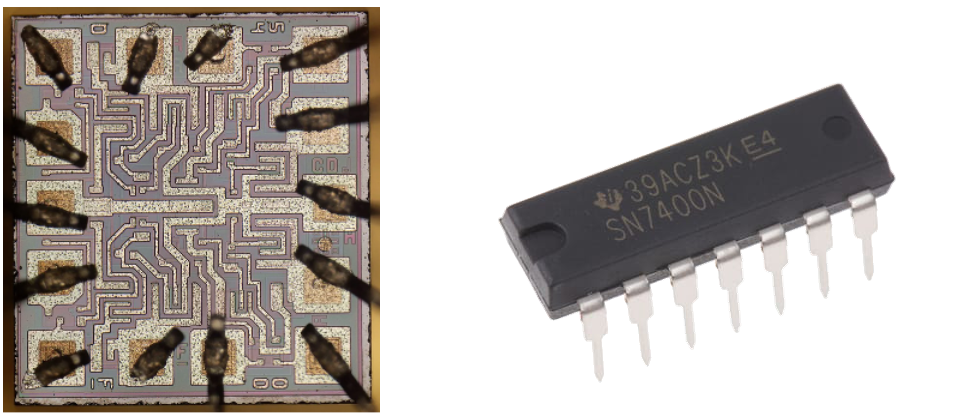
\includegraphics[width=0.40\textwidth]{lab-reports/Schematics-and-graphics/SN7400N.png}
\caption{Fotografia del DIE e \textit{package} plastico DIP \textit{(Dual Inline Package)} dell'integrato con 2 porte NAND SN7400N}
\label{fig:integrated_nand}
\end{center}
\end{figure}

\subsection{Transistor di interfaccia PN2222A}
Testo

\subsection{Integrato di \textit{sample holding} LF398}
Testo

\subsection{Scheda a microcontrollore}
Nell'ultima fase dell'esperienza di laboratorio verrà realizzato un semplice sistema di registrazione dei valori acquisiti utilizzando un microcontrollore \textit{Atmel ATmega328P} basato sull'architettura Harvard RISC a 8 bit interfacciato con un lettore di schede microSD. Questo MCU viene impiegato con un oscillatore esterno al quarzo a 16 MHz per il clock, dispone di 32 KB di memoria ISP flash e nel nostro caso è installato su una scheda Arduino che ospita anche un secondo microcontrollore \textit{Atmel ATmega16u2} con funzione di interfaccia di programmazione USB. La funzione di questo dispositivo è quella di leggere lo stato delle uscite dei J-K, corrispondente alla rappresentazione binaria del segnale campionato, e di scrivere su un file salvato una scheda microSD a cui è connesso mediante una linea seriale SPI.



%%%%%%%%%%%%%%%%%%%%%%%%%%%%%%%%%%%%%%%%%%%%%%%%%%%%%%%%%%%%%
%% Primo Giorno 
%%%%%%%%%%%%%%%%%%%%%%%%%%%%%%%%%%%%%%%%%%%%%%%%%%%%%%%%%%%%%

\section{Caratterizzazione del flip-flop RS}

\begin{figure}[H]%[!ht]
\begin{center}
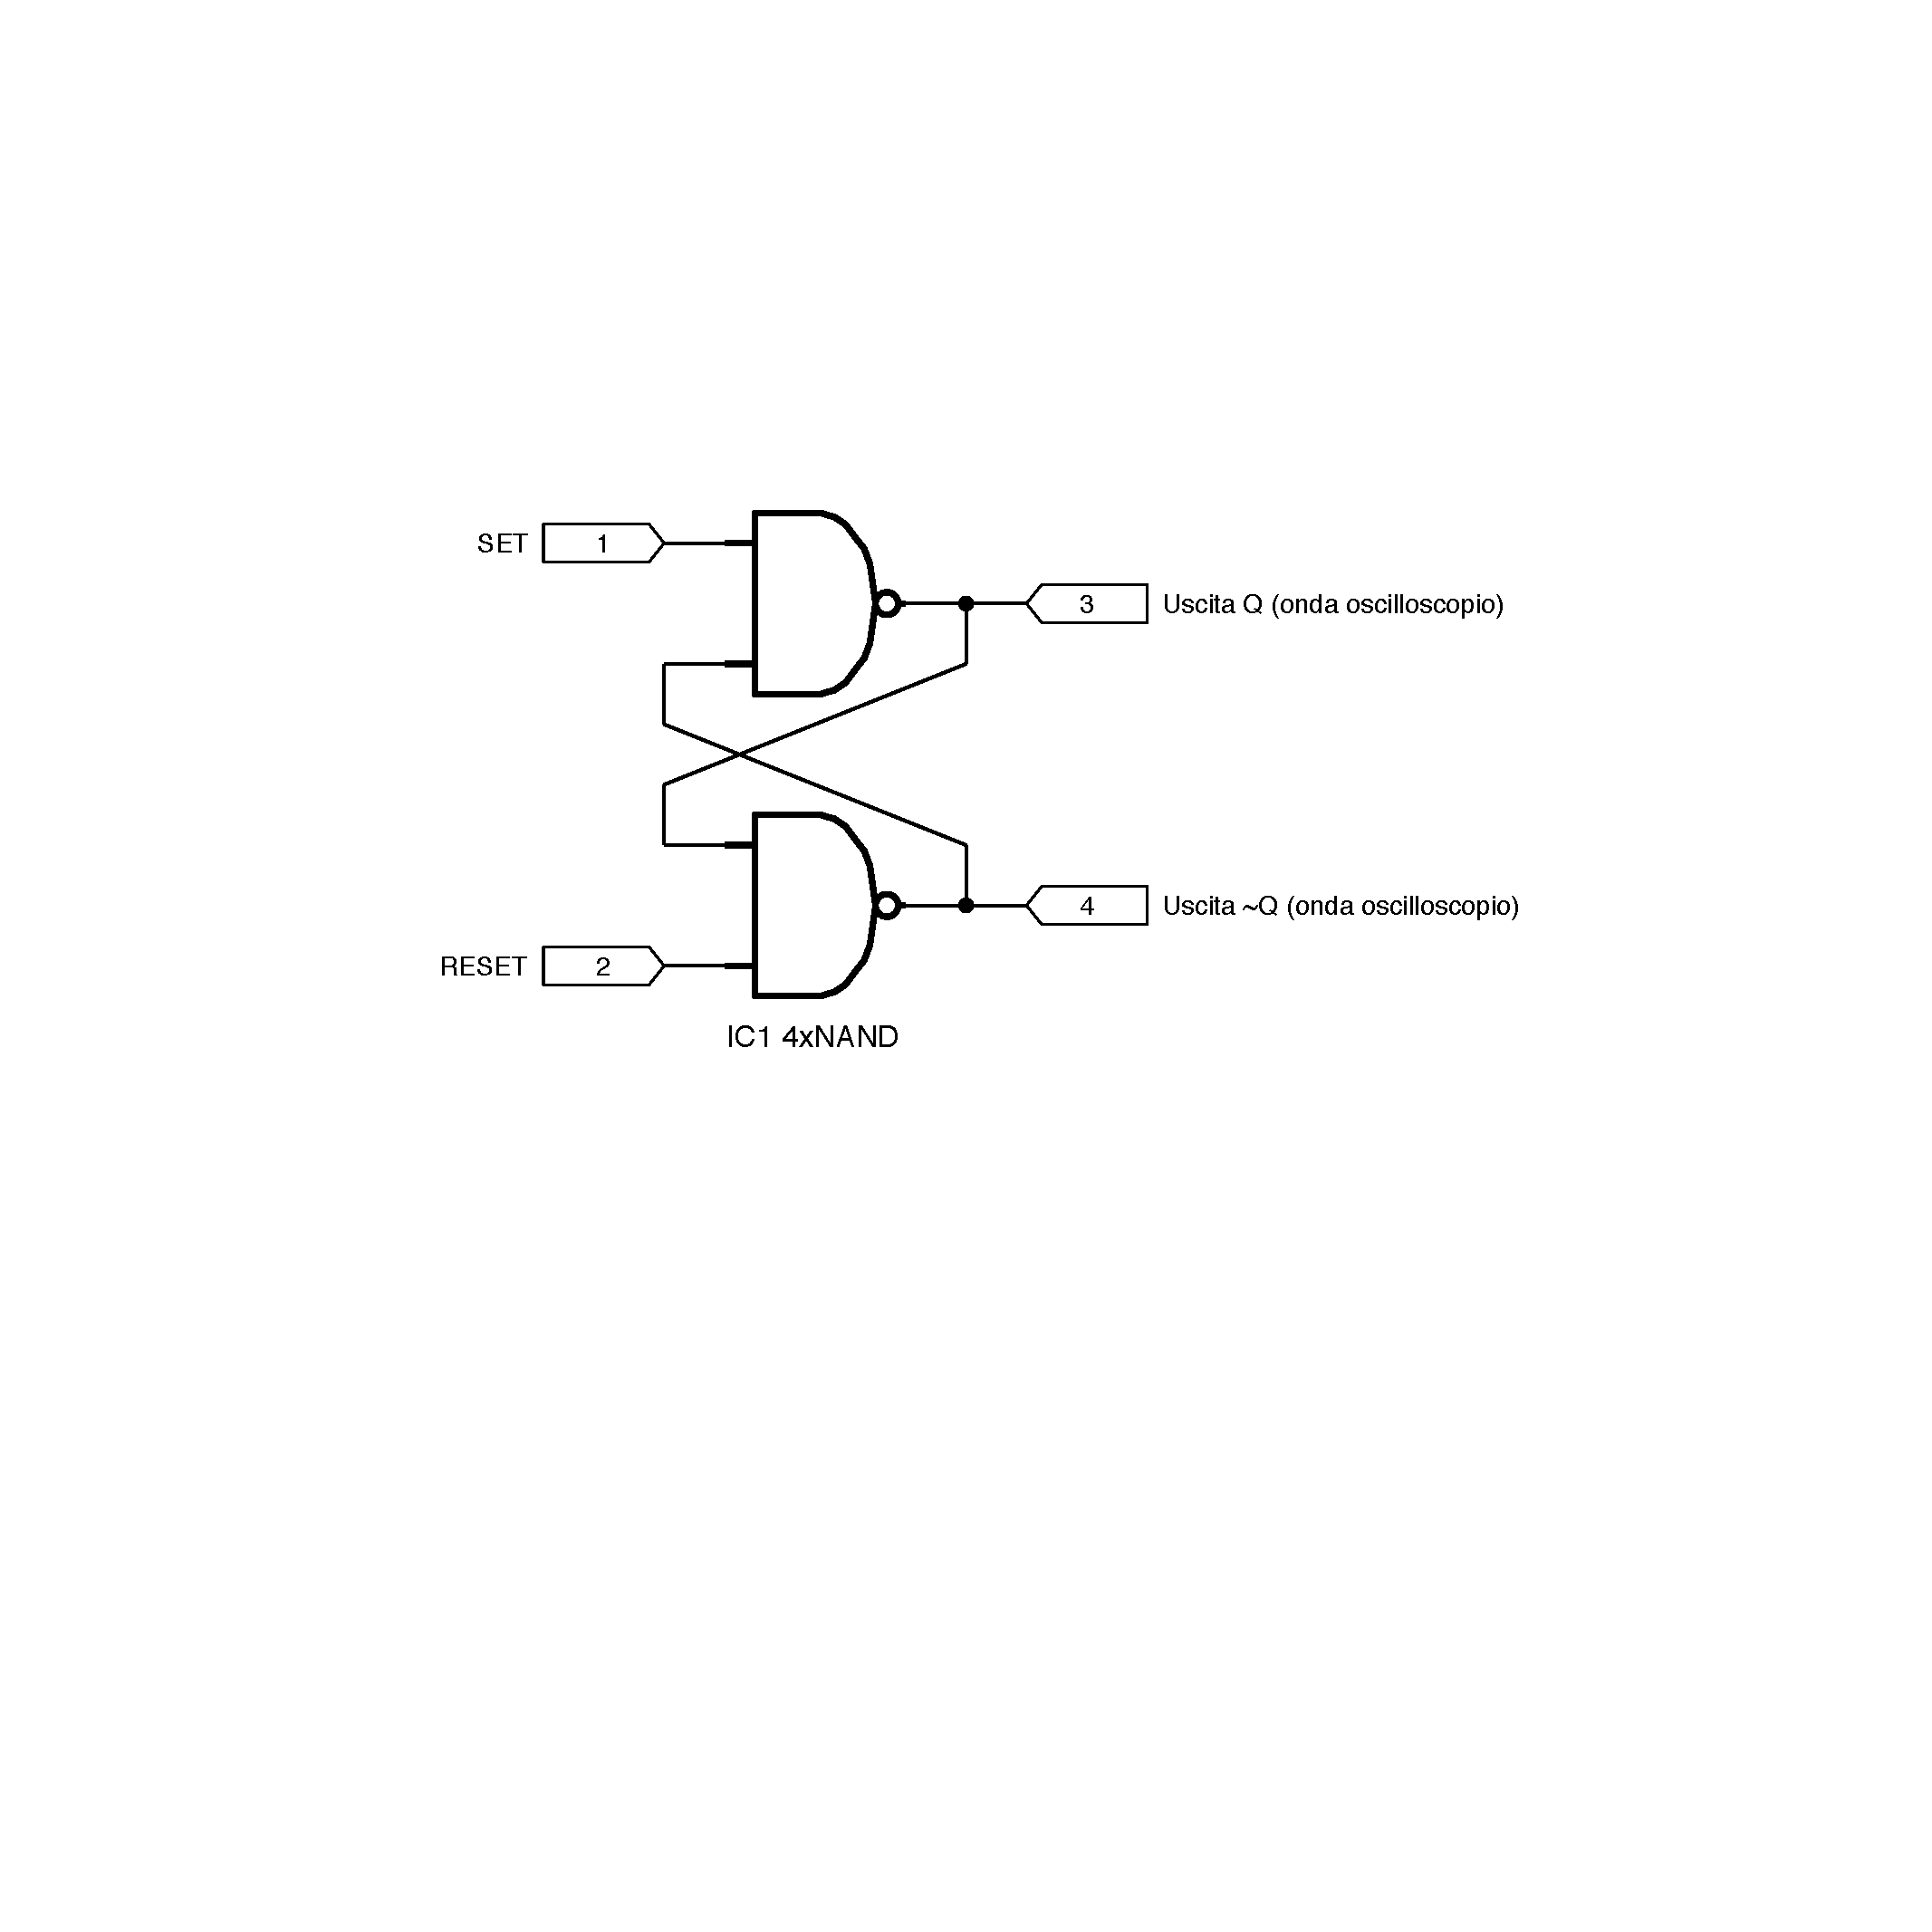
\includegraphics[width=0.30\textwidth]{sch-simulations/digital/output/flip-flop-RS.pdf}
\caption{Logica interna del flip-flop set-reset}
\label{fig:circuit_flip_flop}
\end{center}
\end{figure}

%%%%%%%%%%%%%%%%%%%%%%%%%%%%%%%%%%%%%%%%%%%%%%%%%%%%%%%%%%%%%

\begin{figure}[H]%[!ht]
\begin{center}
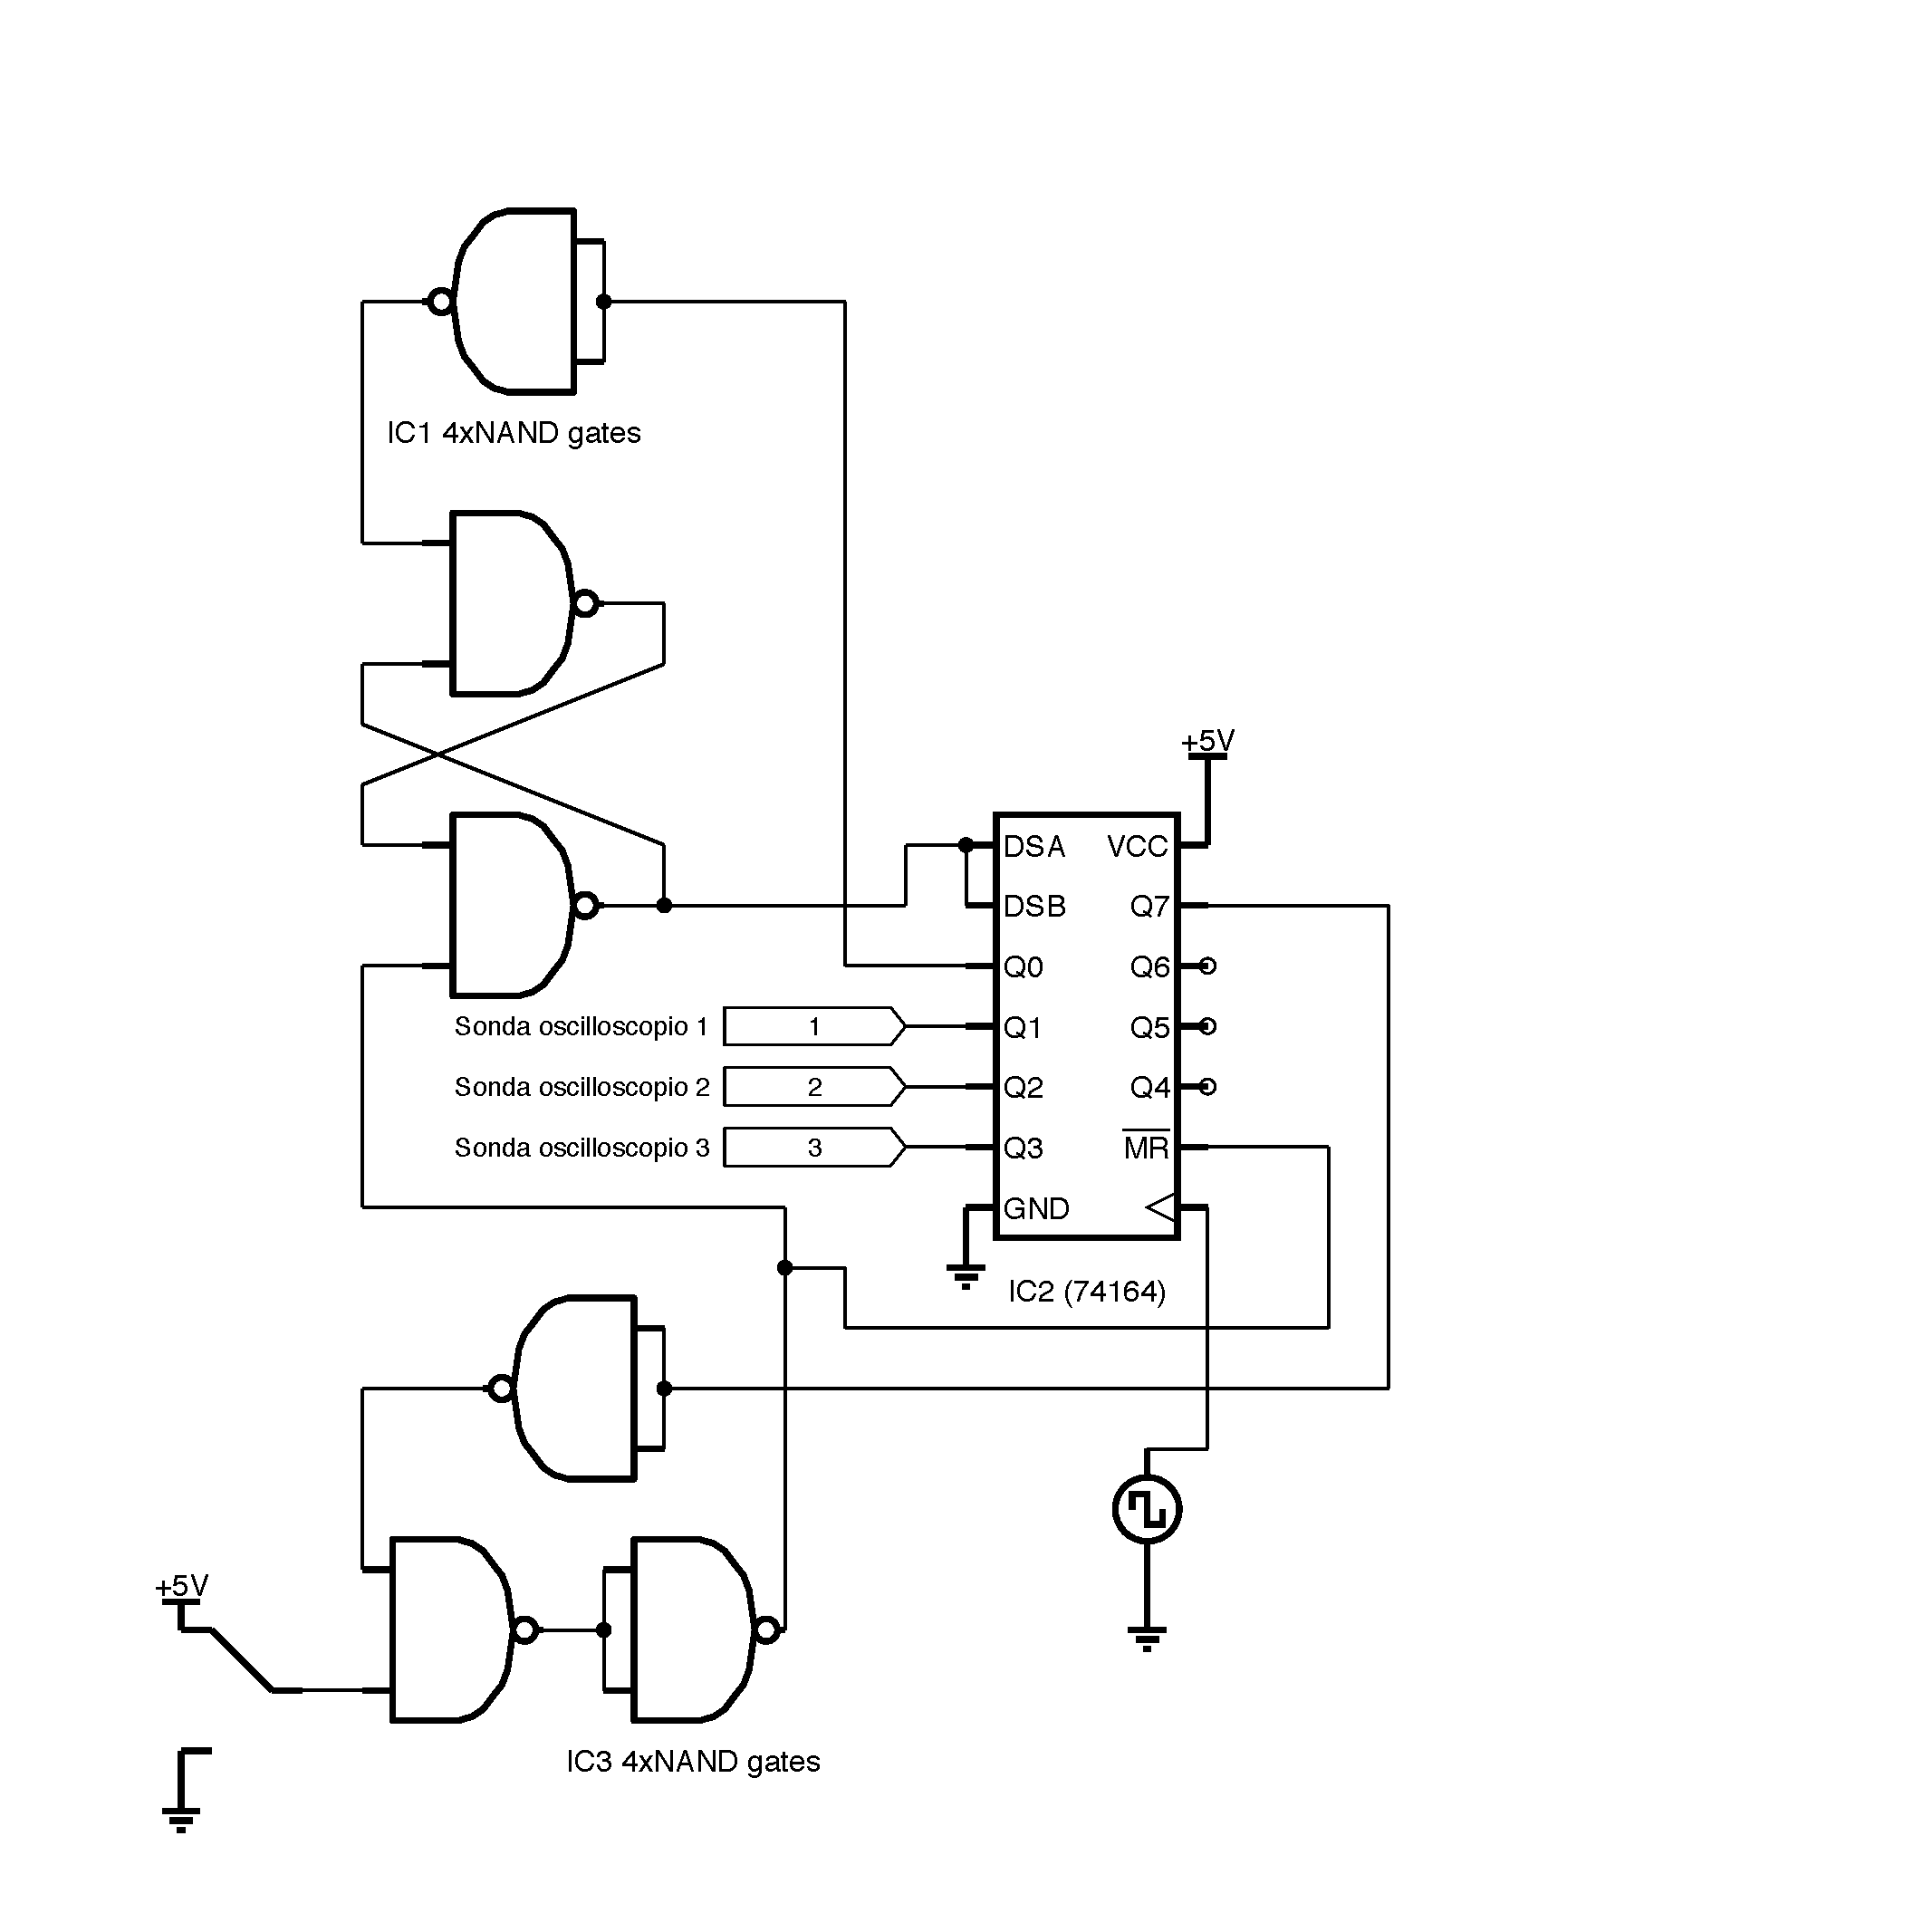
\includegraphics[width=0.54\textwidth]{sch-simulations/digital/output/shift-register.pdf}
\caption{Registro a scorrimento e circuito di controllo}
\label{fig:circuit_shift_register}
\end{center}
\end{figure}


\begin{figure}[H]%[!ht]
\begin{center}
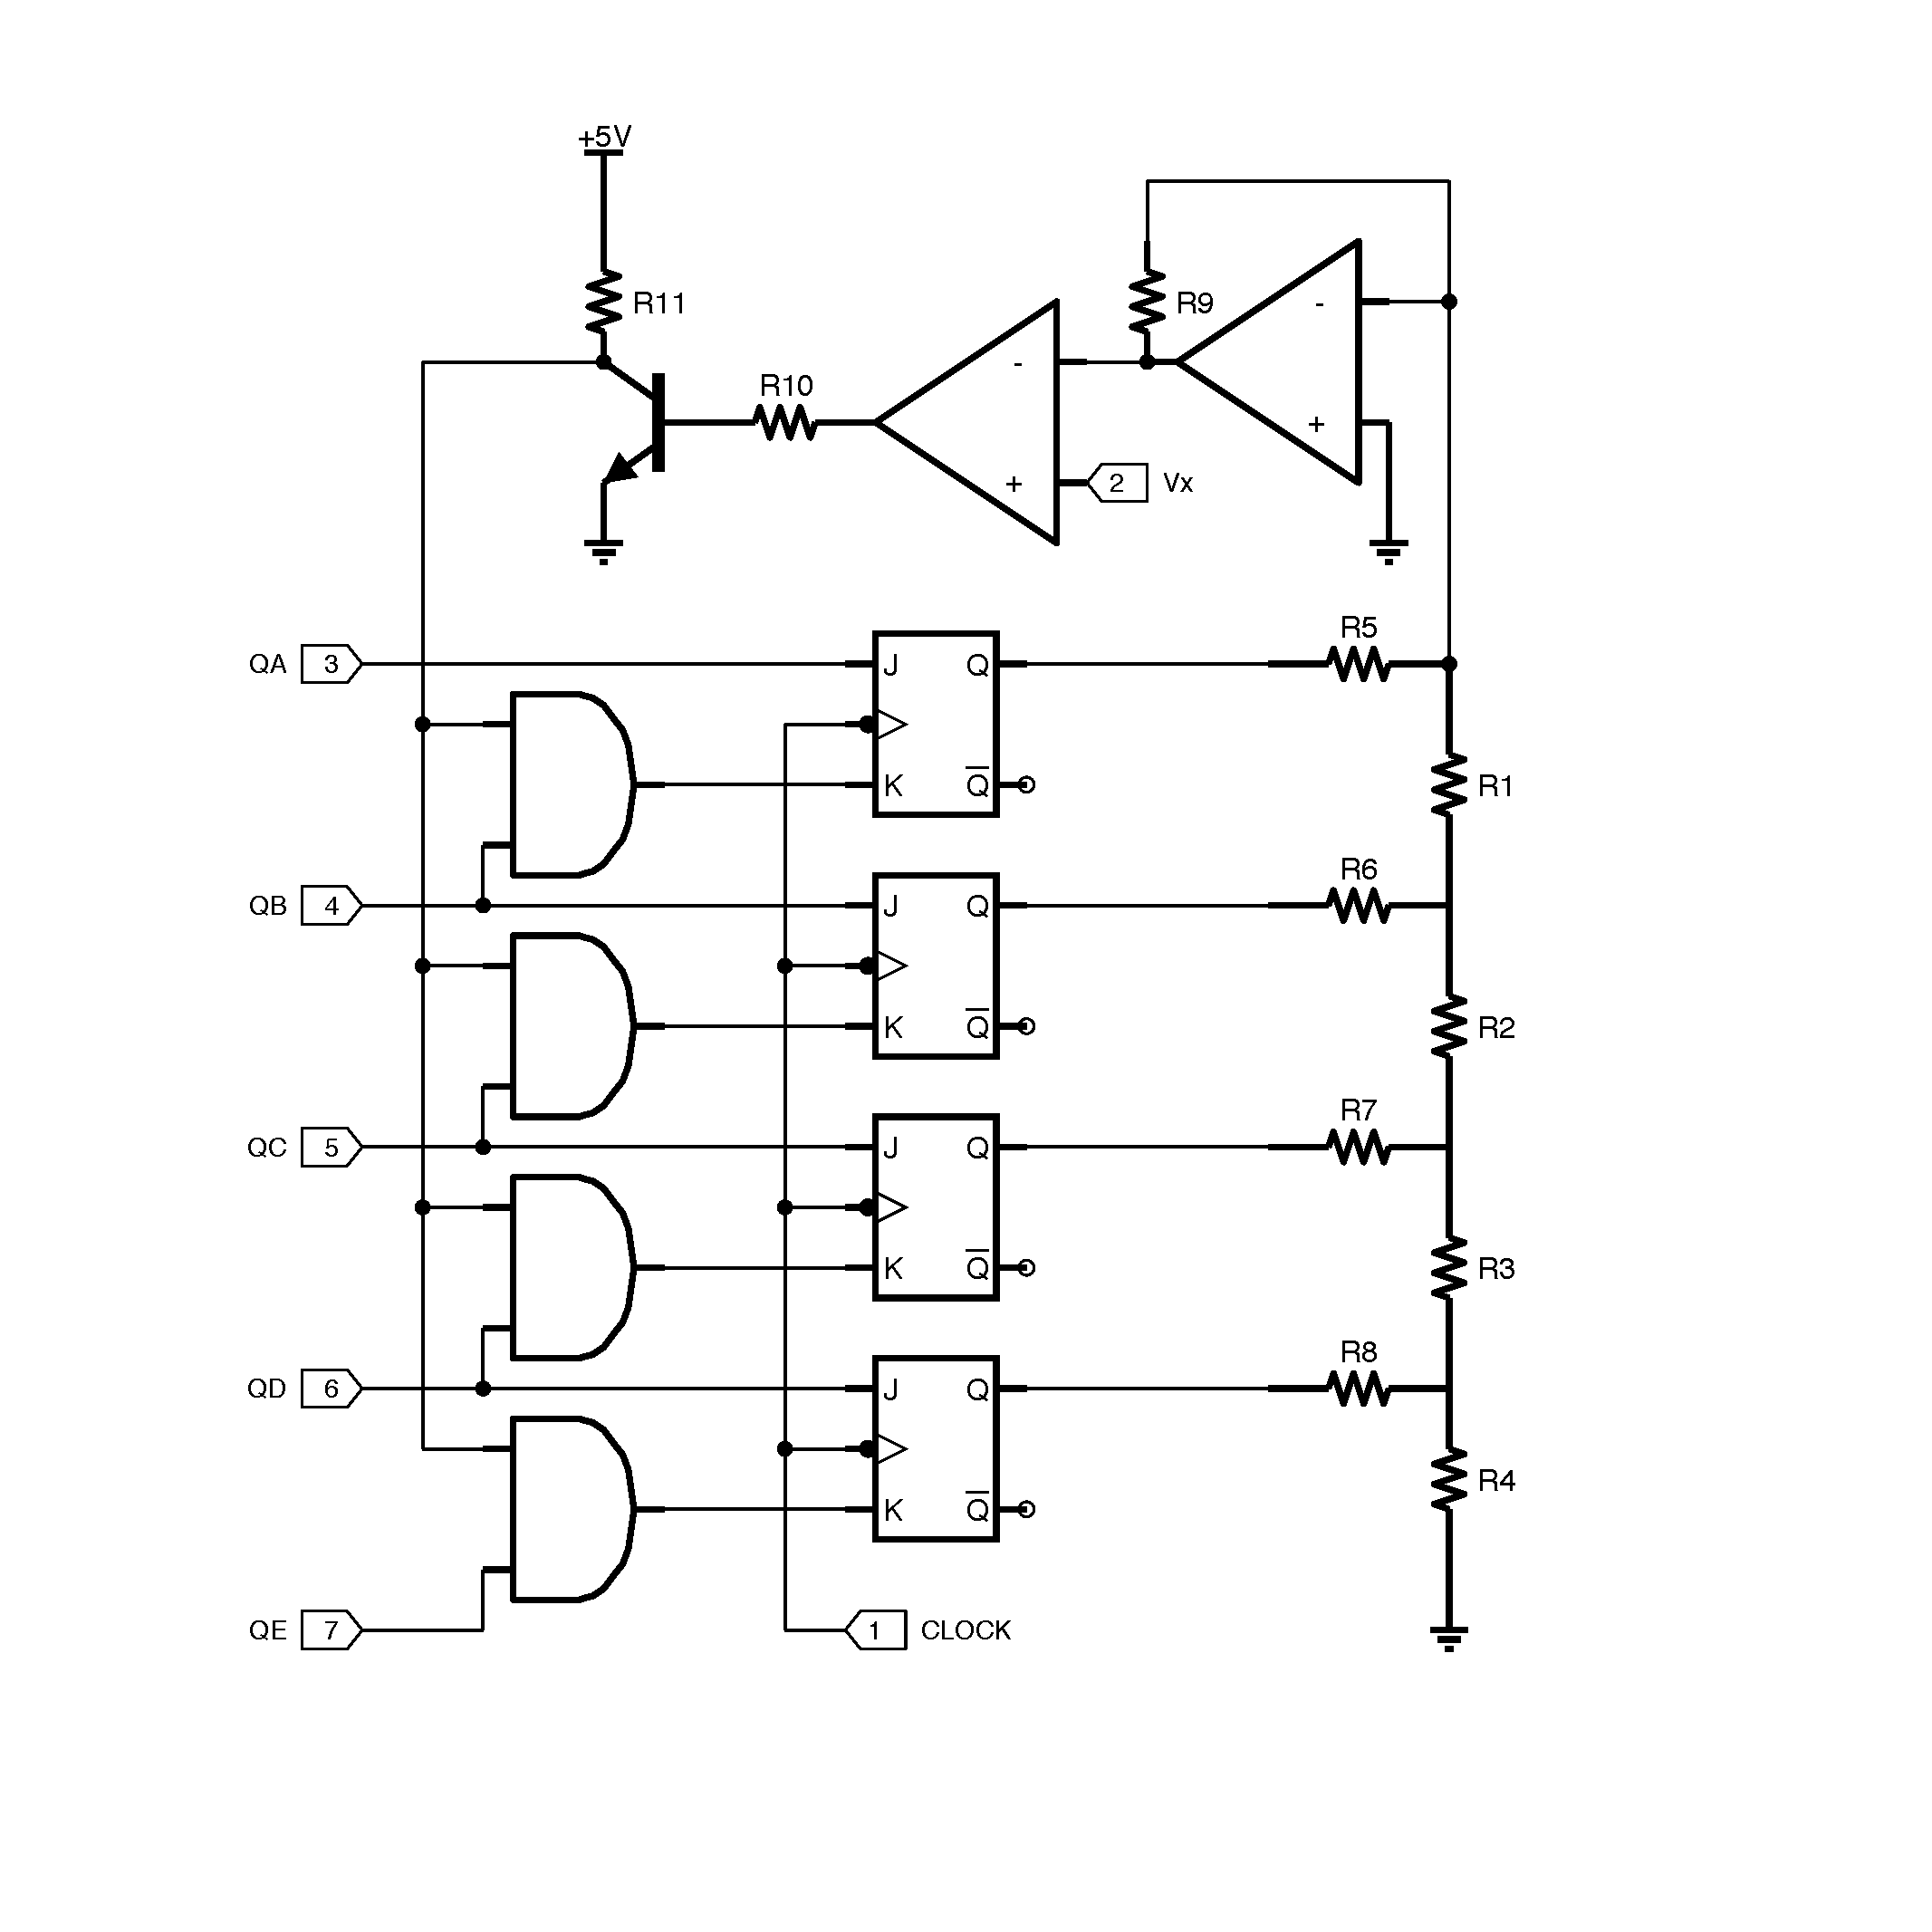
\includegraphics[width=0.40\textwidth]{sch-simulations/digital/output/DAC.pdf}
\caption{DAC}
\label{fig:circuit_shift_register}
\end{center}
\end{figure}


%%%%%%%%%%%%%%%%%%%%%%%%%%%%%%%%%%%%%%%%%%%%%%%%%%%%%%%%%%%%%
%% Secondo Giorno 
%%%%%%%%%%%%%%%%%%%%%%%%%%%%%%%%%%%%%%%%%%%%%%%%%%%%%%%%%%%%%

\section{Tabella di verità AND}

\subsection{Misura $V_{IH}$ }

%%%%%%%%%%%%%%%%%%%%%%%%%%%%%%%%%%%%%%%%%%%%%%%%%%%%%%%%%%%%%

\section{Tabella di verità JK}

\begin{figure}[t]%[t]
\centering
\begin{center}
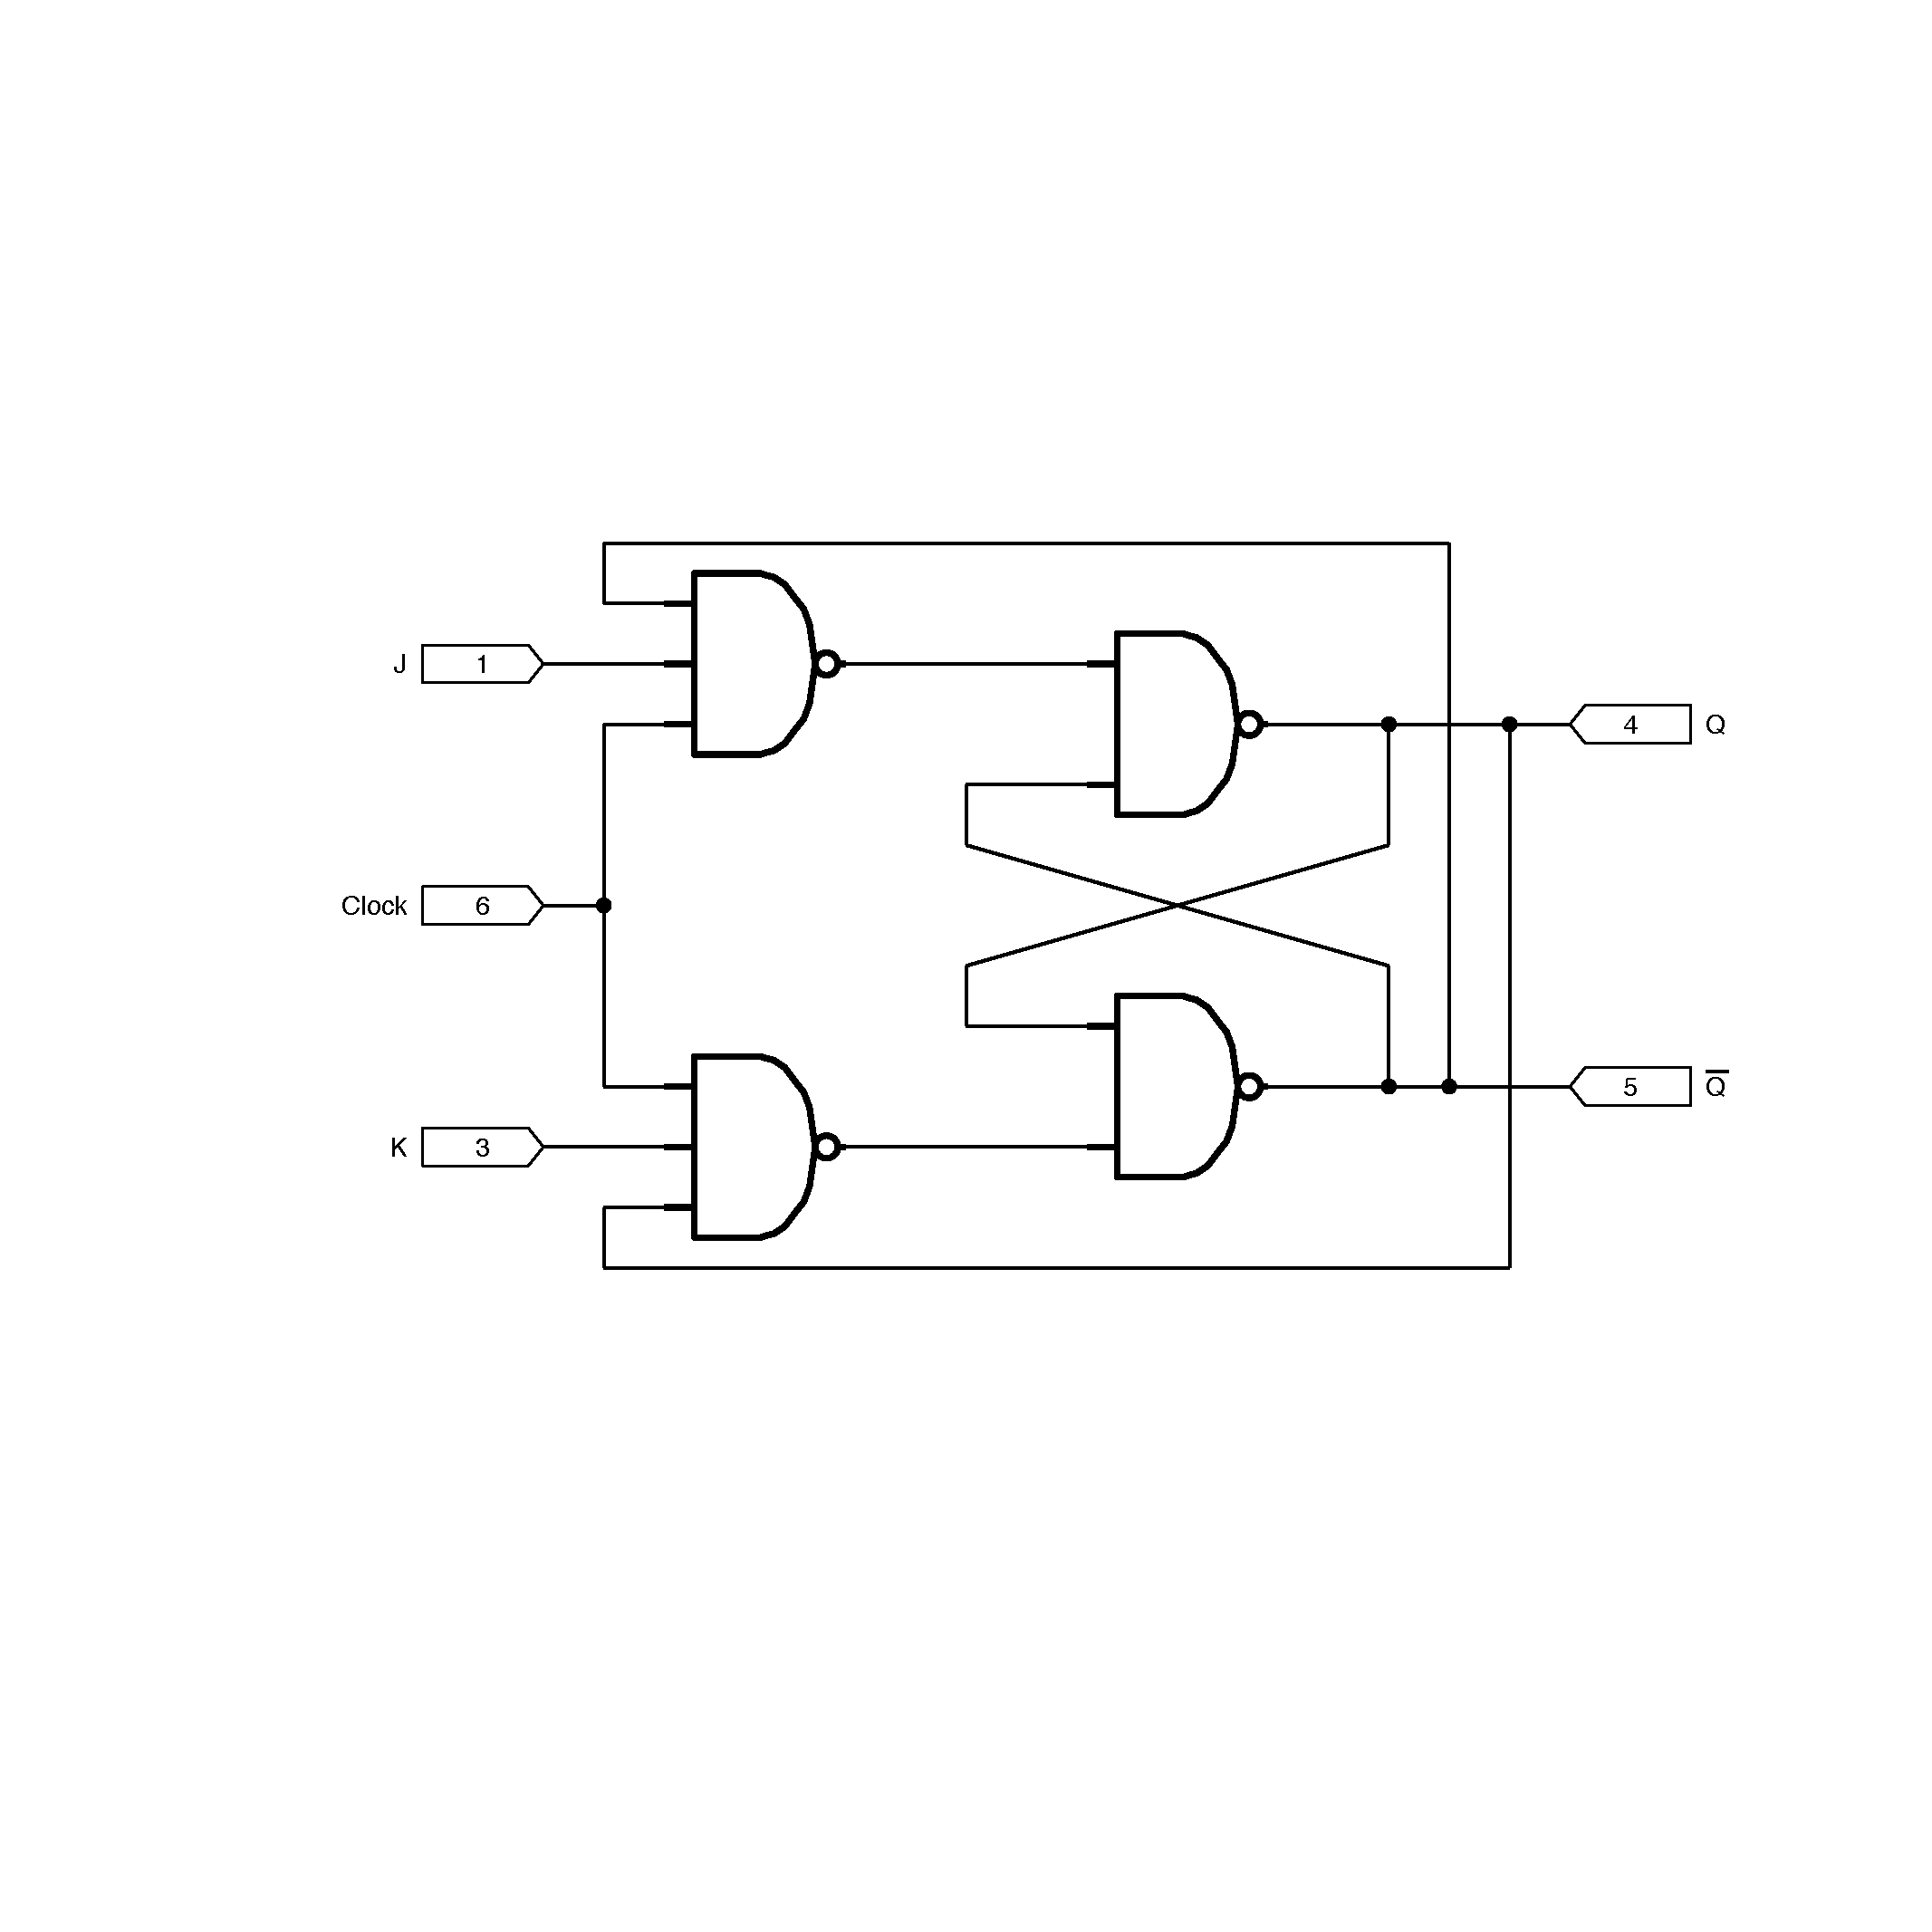
\includegraphics[width=0.40\textwidth]{sch-simulations/digital/output/flip-flop-JK.pdf}
\end{center}
\caption{Logica interna del flip-flop JK}
\label{fig:circuit_JK}
\end{figure}

%%%%%%%%%%%%%%%%%%%%%%%%%%%%%%%%%%%%%%%%%%%%%%%%%%%%%%%%%%%%%
%% Terzo Giorno 
%%%%%%%%%%%%%%%%%%%%%%%%%%%%%%%%%%%%%%%%%%%%%%%%%%%%%%%%%%%%%

\begin{figure*}[t]%[t]
\centering
\begin{center}
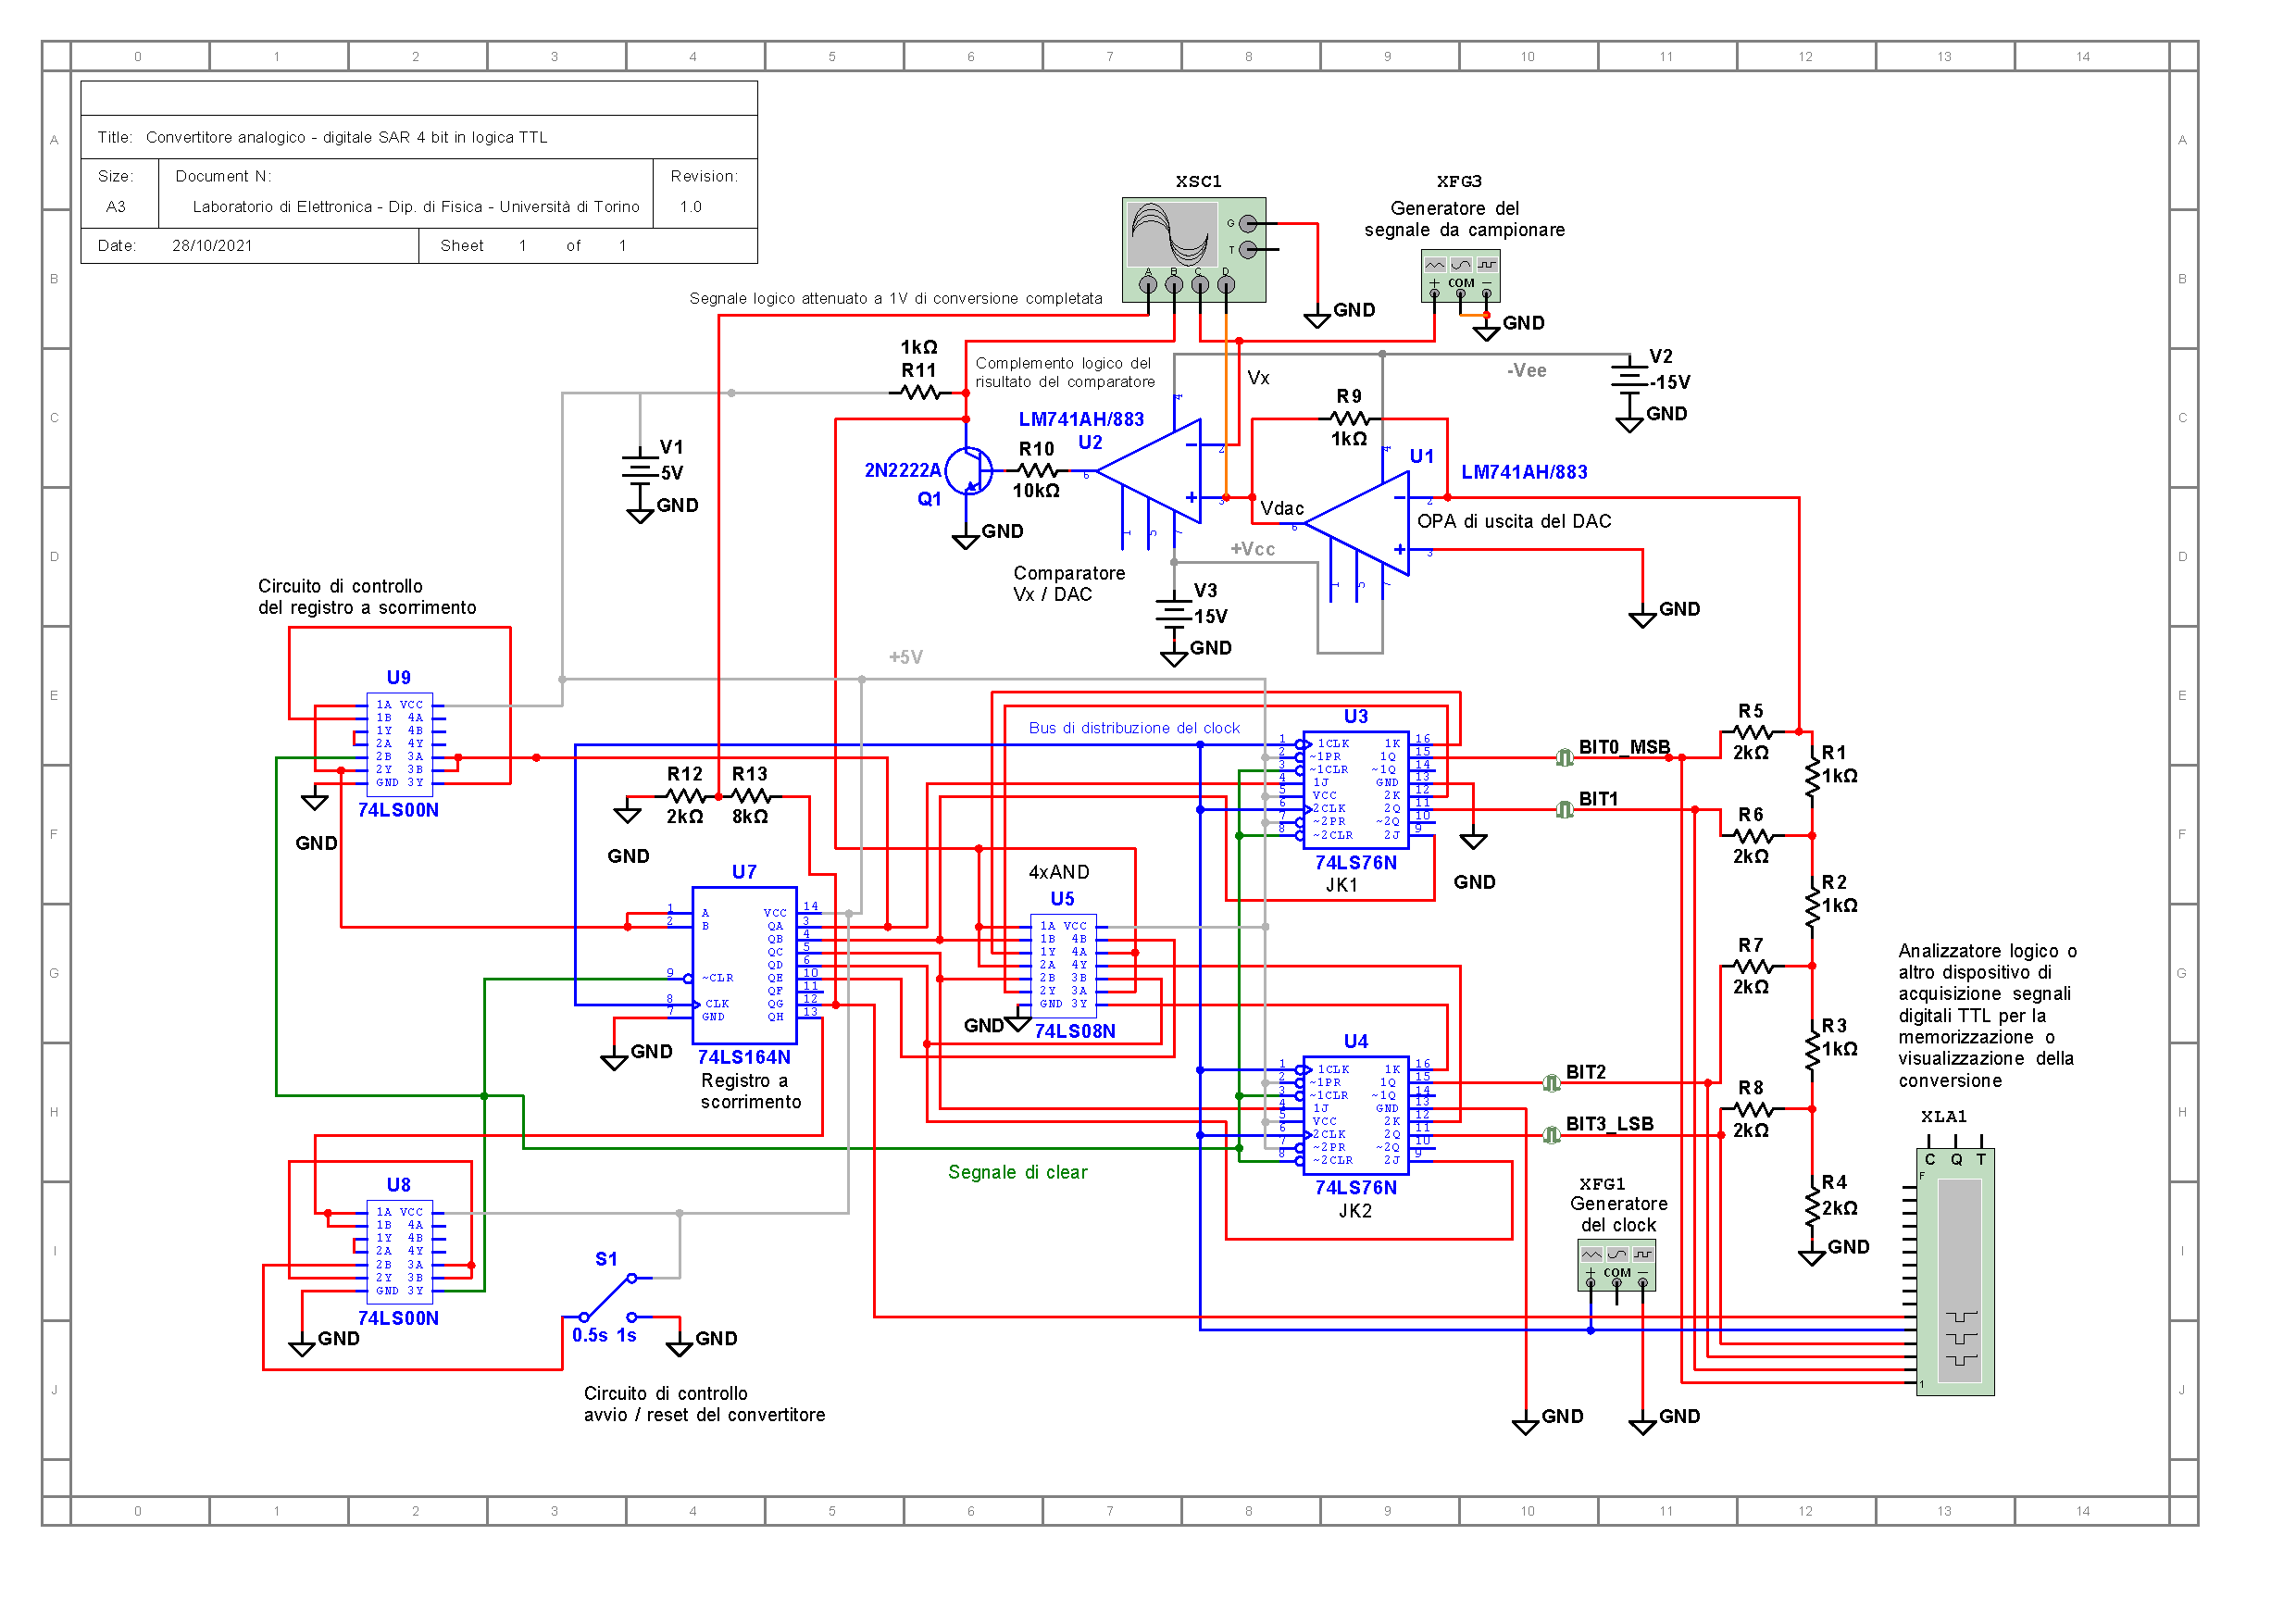
\includegraphics[trim = {0 0 50 0}, width=1.40\textwidth, angle=90]{sch-simulations/digital/output/Schema_convertitore_completo.pdf}
\end{center}
\caption{Schema elettrico completo del convertitore ADC SAR 4 bit}
\label{fig:circuit_sarCompleteSchematic}
\end{figure*}



%%%%%%%%%%%%%%%%%%%%%%%%%%%%%%%%%%%%%%%%%%%%%%%%%%%%%%%%%%%%%
%% Appendice
%%%%%%%%%%%%%%%%%%%%%%%%%%%%%%%%%%%%%%%%%%%%%%%%%%%%%%%%%%%%%


\begin{appendices}

\section{Oscillatore ad anello}

\begin{figure}[H]%[!ht]
\begin{center}
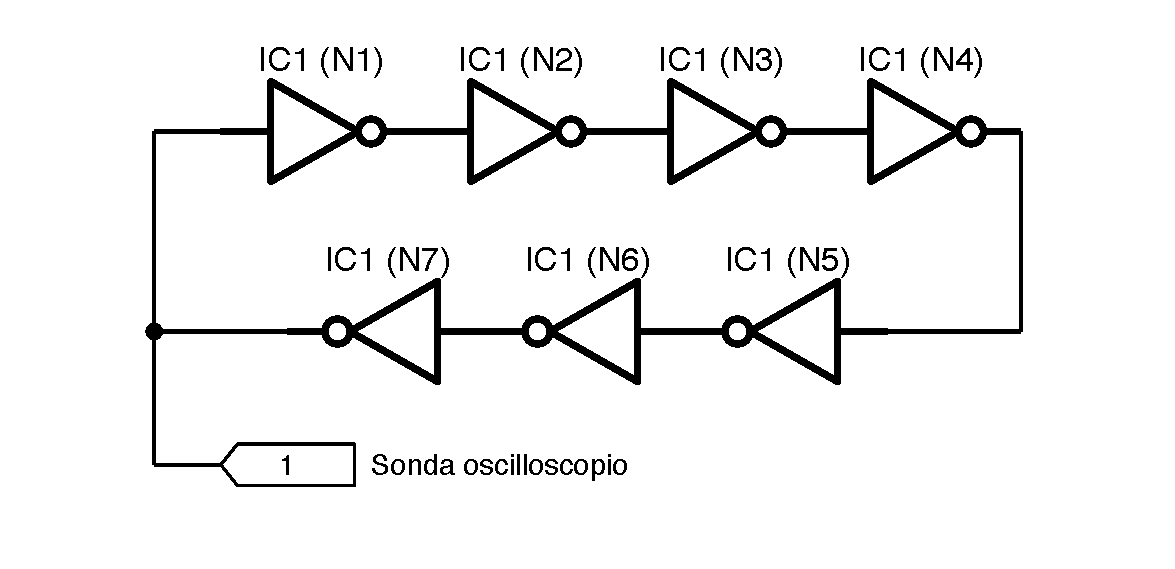
\includegraphics[width=0.40\textwidth]{sch-simulations/digital/output/ring-osc-logic.pdf}
\caption{Circuito equivalente dell'oscillatore ad anello}
\label{fig:circuit_ring_oscillator}
\end{center}
\end{figure}

\begin{figure}[H]%[!ht]
\begin{center}
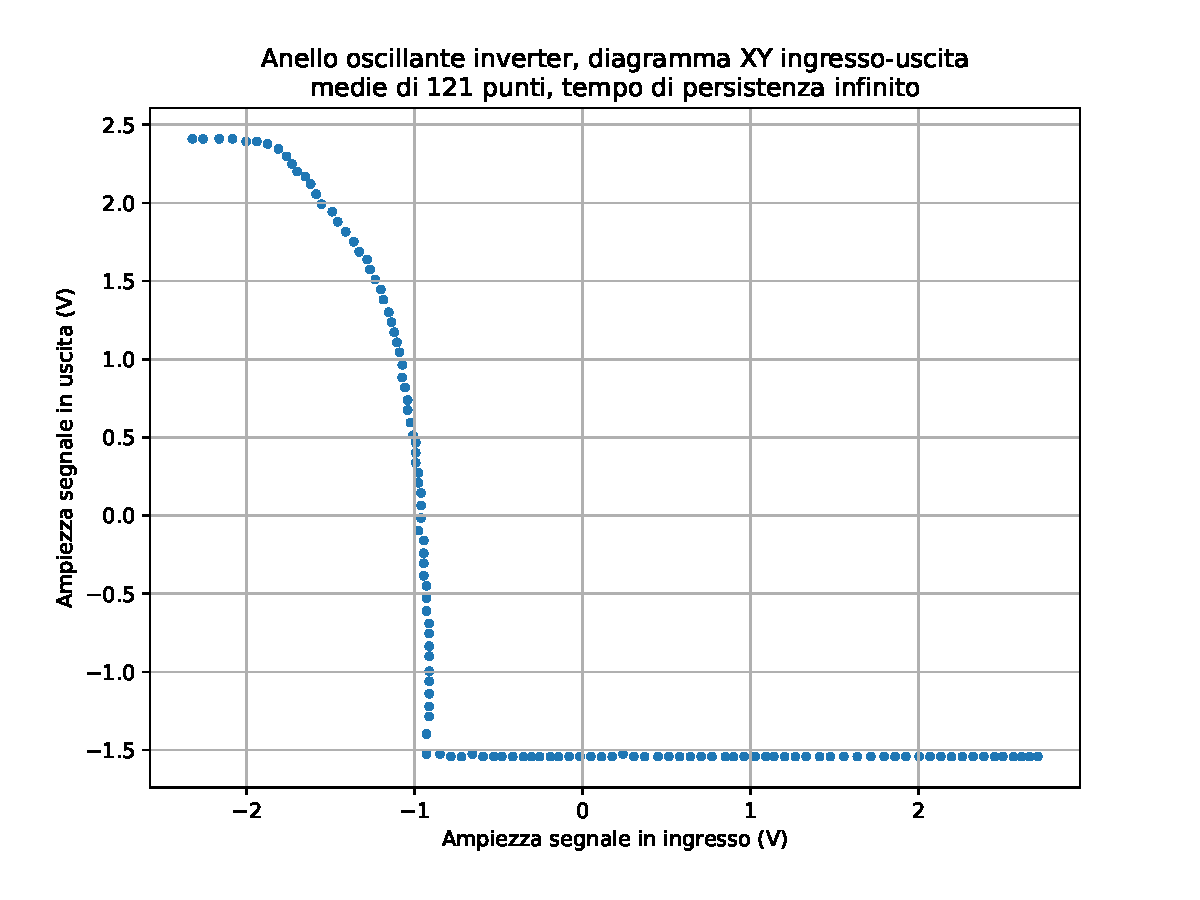
\includegraphics[width=0.48\textwidth]{analysis/output/inverter_ring_xy.pdf}
\caption{Studio dell'oscillatore ad anello}
\label{fig:inverter_ring_xy}
\end{center}
\end{figure}

%%%%%%%%%%%%%%%%%%%%%%%%%%%%%%%%%%%%%%%%%%%%%%%%%%%%%%%%%%%%%

\section{Caratterizzazione transistor npn}


\end{appendices}

%%%%%%%%%%%%%%%%%%%%%%%%%%%%%%%%%%%%%%%%%%%%%%%%%%%%%%%%%%%%%
%% Indice e Bibliografia 
%%%%%%%%%%%%%%%%%%%%%%%%%%%%%%%%%%%%%%%%%%%%%%%%%%%%%%%%%%%%%

\clearpage
\newpage

\tableofcontents % Indice

\newpage

\printbibliography % Bibliografia

\end{document}